% === [ Appendices ] ===========================================================

\appendix
\setcounter{secnumdepth}{0}
\section{Appendices}
\setcounter{secnumdepth}{3}
\renewcommand{\thesubsection}{\Alph{subsection}}

% --- [ Project Initiation Document ] ------------------------------------------

\subsection{Project Initiation Document}


\includepdf[pages=-]{appendices/PID.pdf}

% --- [ Certificate of Ethics Review ] -----------------------------------------

\subsection{Certificate of Ethics Review}


\includepdf[pages=-]{appendices/ethics_review.pdf}

% --- [ Gantt Chart ] ----------------------------------------------------------

\subsection{Initial and Final Gantt Charts}

\begin{figure}[htbp]
	\begin{center}
		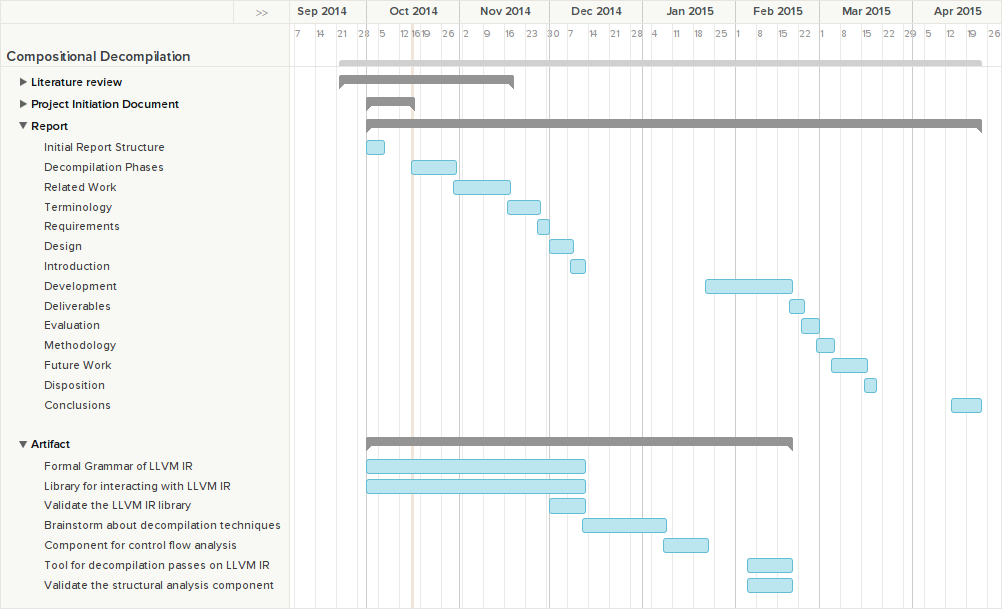
\includegraphics[angle=270, width=0.9\textwidth]{appendices/gantt_initial.png}
		\caption{Initial Gantt chart.}
	\end{center}
\end{figure}

% TODO: Add final Gantt chart.

\pagebreak

% --- [ The REIL Instruction Set ] ---------------------------------------------

\subsection{The REIL Instruction Set}
\label{app:reil_instructions}

\lstinputlisting[language=reil, style=nasm, caption={A full definition of the REIL instruction set. \label{lst:reil_instructions}}]{appendices/reil_instruction_set.asm}

\pagebreak

% --- [ Patch for Unnamed Basic Blocks of LLVM ] -------------------------------

\subsection{Patch for Unnamed Basic Blocks of LLVM}
\label{app:unnamed_patch}

The following patch ensures that the assembly printer of LLVM 3.6.0 always prints the generated names of unnamed basic blocks.

\lstinputlisting[language=diff, style=diff, caption={Always print the generated names of unnamed basic blocks. \label{lst:unnamed_patch}}]{appendices/unnamed.patch}

\pagebreak

% --- [ Control Flow Analysis Example ] ----------------------------------------

\subsection{Control Flow Analysis Example}
\label{app:control_flow_analysis_example}

This section provides a step-by-step demonstration of how the control flow analysis is conducted by analysing the \texttt{stmt} function of the c4 compiler\footnote{C in four functions: \url{https://github.com/rswier/c4}}. The control flow analysis operates exclusively on CFGs, which are generated by a set of components prior to the control flow analysis stage. Firstly, the C source code of the c4 compiler is translated into LLVM IR by the Clang compiler of the front-end. Secondly, the LLVM IR is optionally optimized by the \texttt{opt} tool of the LLVM compiler framework. Lastly, a CFG is generated for each function of the LLVM IR using the \texttt{ll2dot} tool.

The control flow analysis stage uses subgraph isomorphism search algorithms to locate isomorphisms of the graph representations of high-level control flow primitives in the CFG of a given function, as further described in section \ref{sec:design_control_flow_analysis}. The CFG is simplified by recursively replacing the identified subgraphs with single nodes until the entire CFG has been reduced into a single node. By recoding the node names of the identified subgraph isomorphisms and the name of their corresponding high-level control flow primitives, a structured CFG may be produced in which all nodes are known to belong to a high-level control flow primitive.

The pseudo-code and graph representations of the supported high-level control flow primitives are presented in figure \ref{fig:graph_representations} of section \ref{sec:control_flow_analysis}. Should the control flow analysis fail to reduce a CFG into a single node, the CFG is considered irreducible with regards to the supported high-level control flow primitives; in which case a structured CFG cannot be produced.

For this demonstration, the CFG of the \texttt{stmt} function is the starting point of the control flow analysis stage. The first step of the control flow analysis recursively locates subgraph isomorphisms of the graph representation of pre-test loops (see figure \ref{fig:pre_test_graph_representation}) in the original CFG of the \texttt{stmt} function, and replaces these subgraphs with single nodes as illustrated in figure \ref{fig:step_1}.

\begin{figure}[htbp]
	\centering
	\begin{subfigure}[t]{0.45\textwidth}
		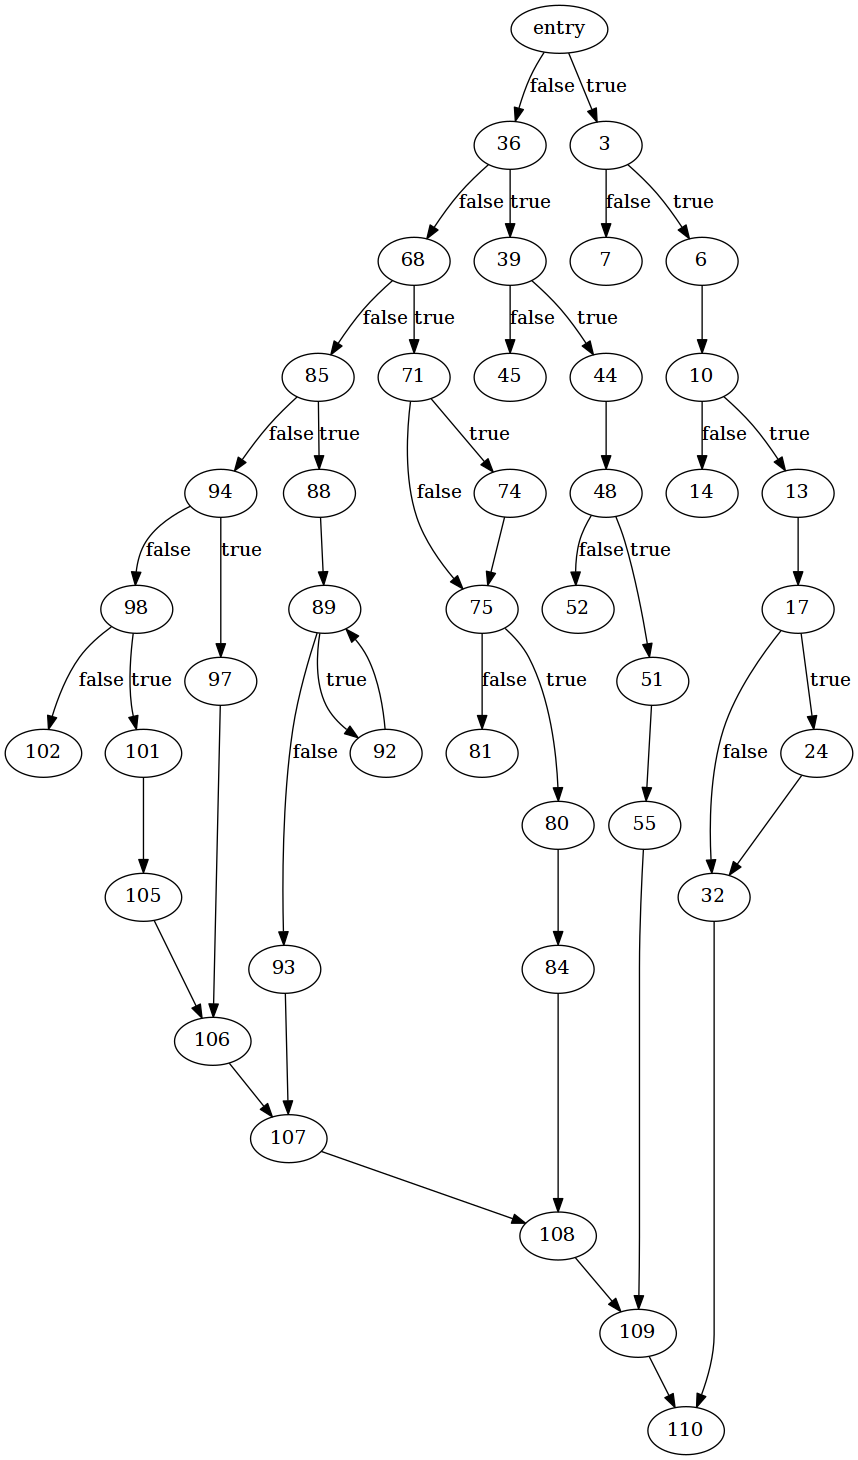
\includegraphics[width=\textwidth]{appendices/stmt_example/stmt_0.png}
	\end{subfigure}
	\qquad
	\begin{subfigure}[t]{0.45\textwidth}
		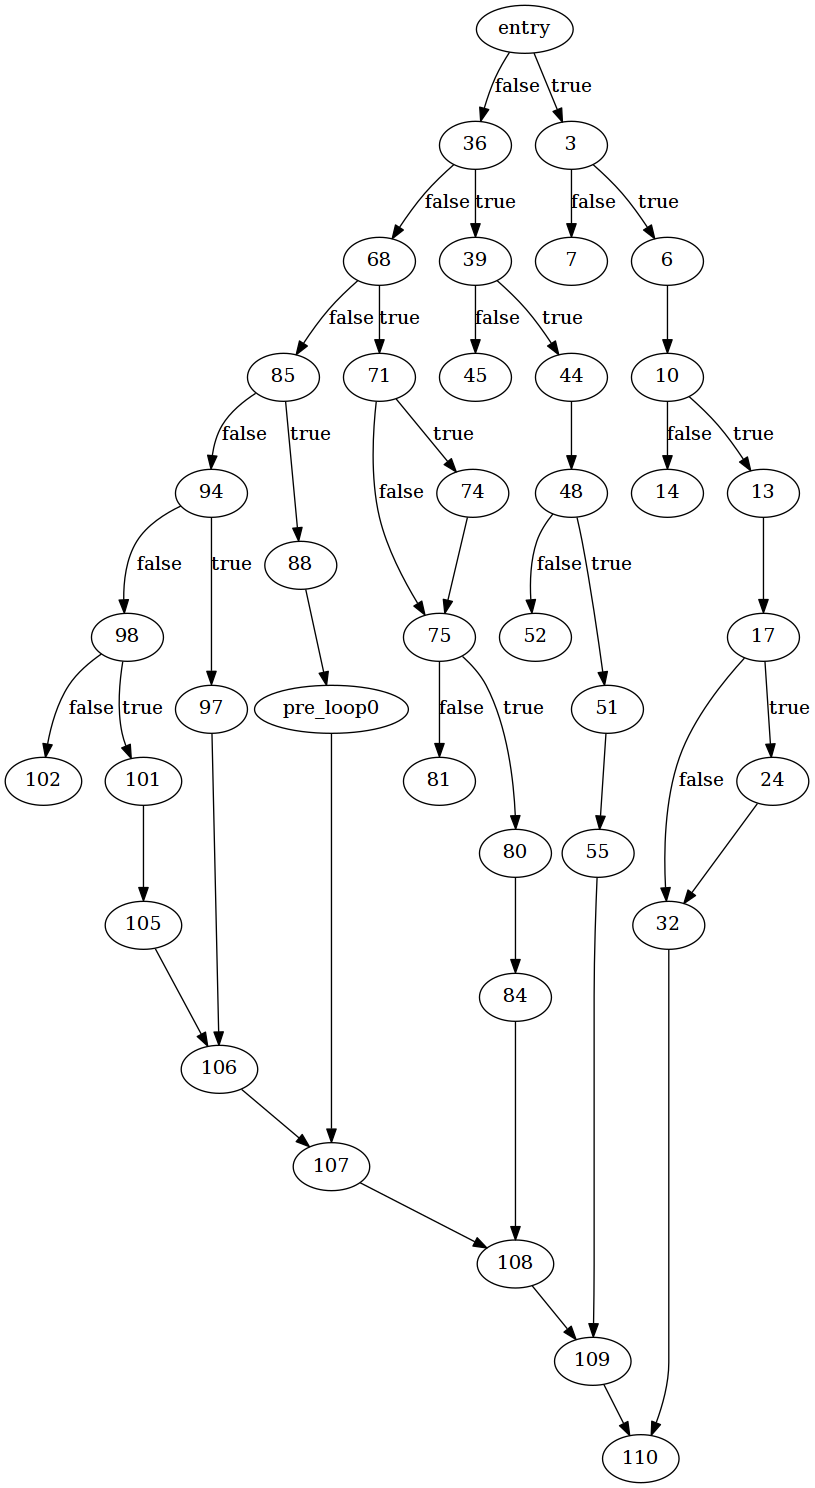
\includegraphics[width=\textwidth]{appendices/stmt_example/stmt_1.png}
	\end{subfigure}
	\caption{\textbf{Step 1}. The original CFG of the \texttt{stmt} function (left) and a simplified CFG (right) after identifying pre-test loops (see figure \ref{fig:pre_test_graph_representation}).}
	\label{fig:step_1}
\end{figure}

The second step further simplifies the CFG of \textbf{step 1} by recursively replacing the subgraph isomorphisms of the graph representation of consecutive statements (see figure \ref{fig:list_graph_representation}) with single nodes, as illustrated in figure \ref{fig:step_2}.

\begin{figure}[htbp]
	\centering
	\begin{subfigure}[t]{0.45\textwidth}
		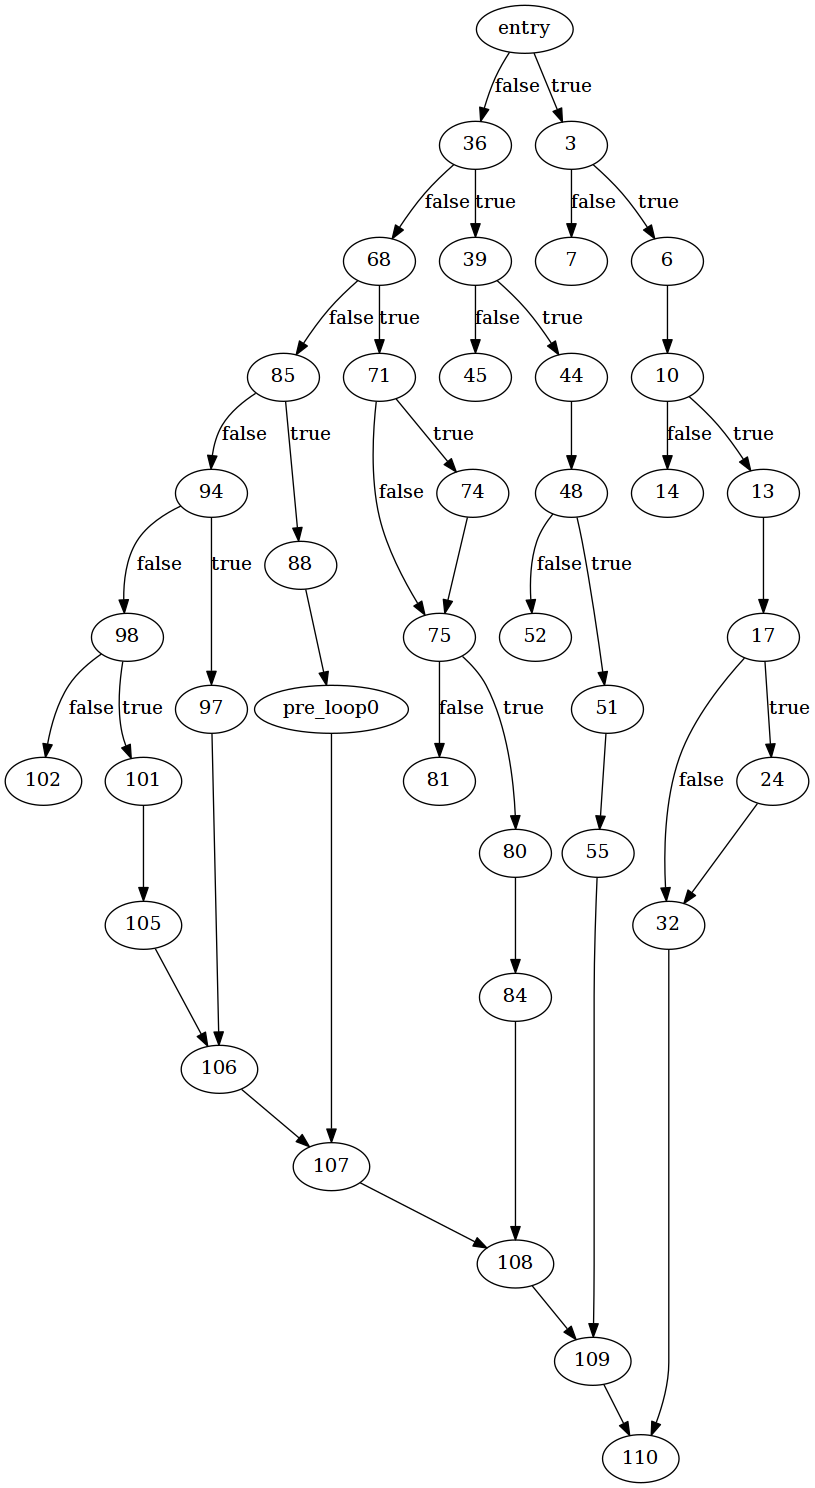
\includegraphics[width=\textwidth]{appendices/stmt_example/stmt_1.png}
	\end{subfigure}
	\qquad
	\begin{subfigure}[t]{0.45\textwidth}
		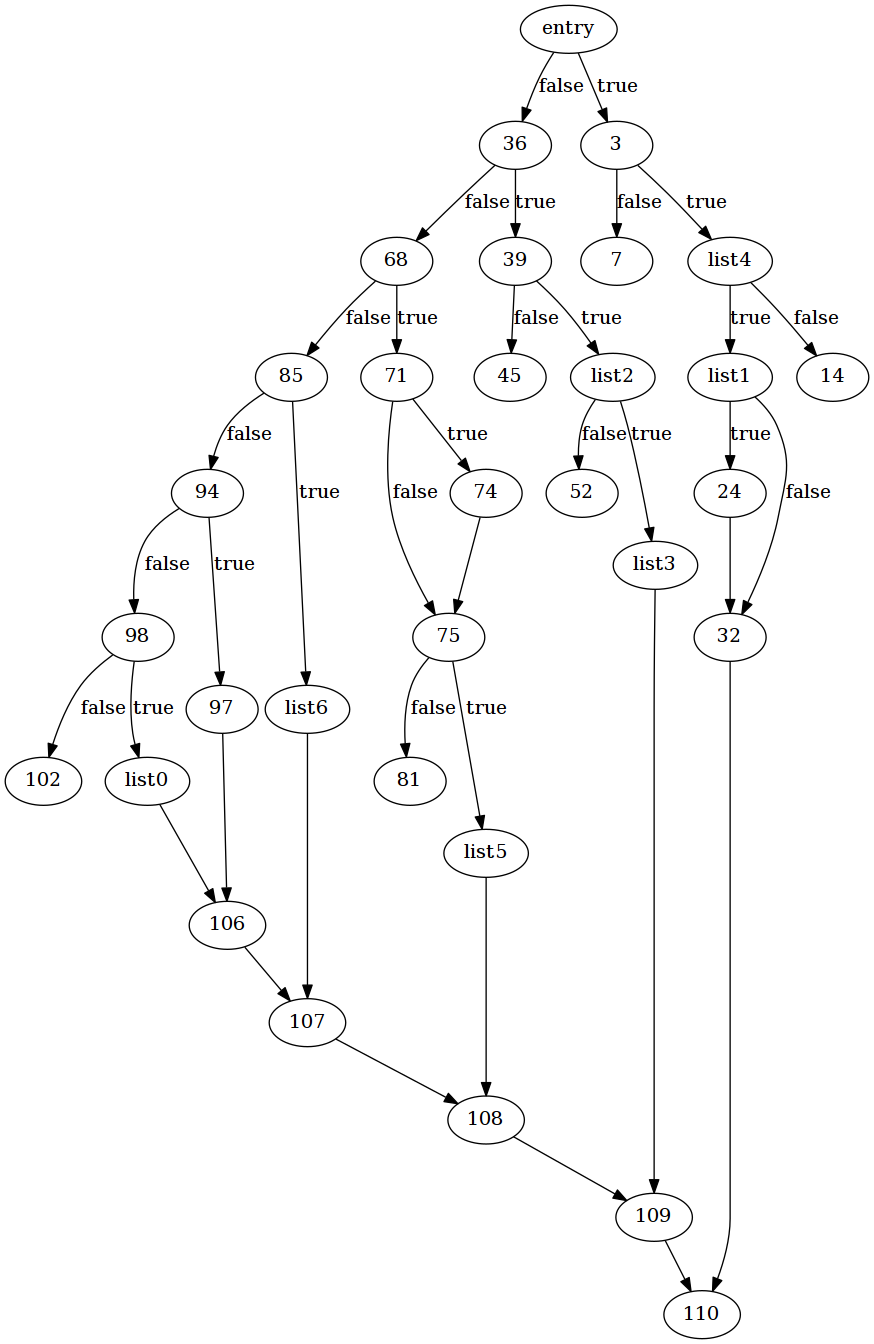
\includegraphics[width=\textwidth]{appendices/stmt_example/stmt_2.png}
	\end{subfigure}
	\caption{\textbf{Step 2}. The CFG from \textbf{step 1} (left) and a simplified CFG (right) after identifying consecutive statements (see figure \ref{fig:list_graph_representation}).}
	\label{fig:step_2}
\end{figure}

The third step further simplifies the CFG of \textbf{step 2} by recursively replacing the subgraph isomorphisms of the graph representation of 1-way conditionals (see figure \ref{fig:if_graph_representation}) with single nodes, as illustrated in figure \ref{fig:step_3}.

\begin{figure}[htbp]
	\centering
	\begin{subfigure}[t]{0.45\textwidth}
		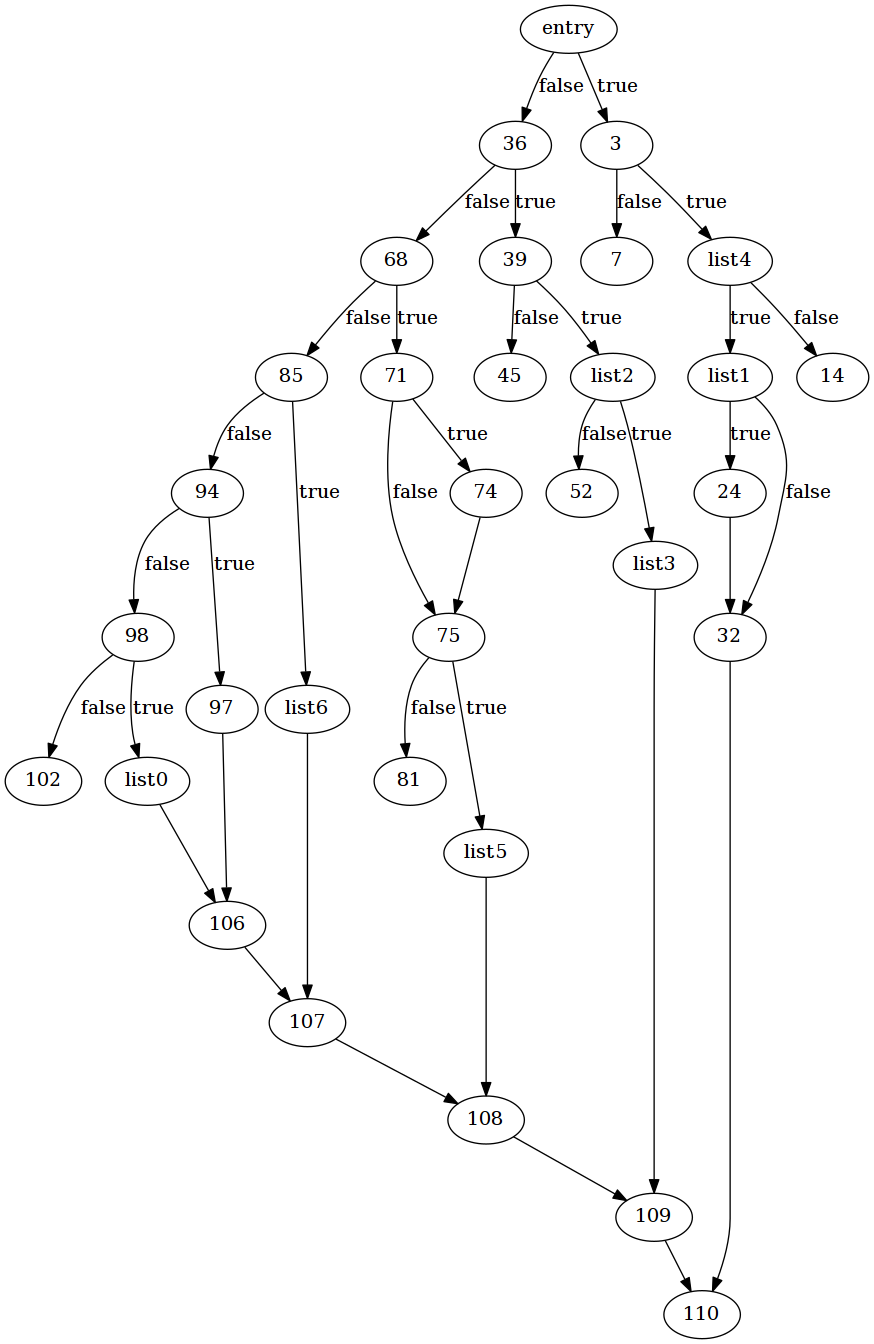
\includegraphics[width=\textwidth]{appendices/stmt_example/stmt_2.png}
	\end{subfigure}
	\qquad
	\begin{subfigure}[t]{0.45\textwidth}
		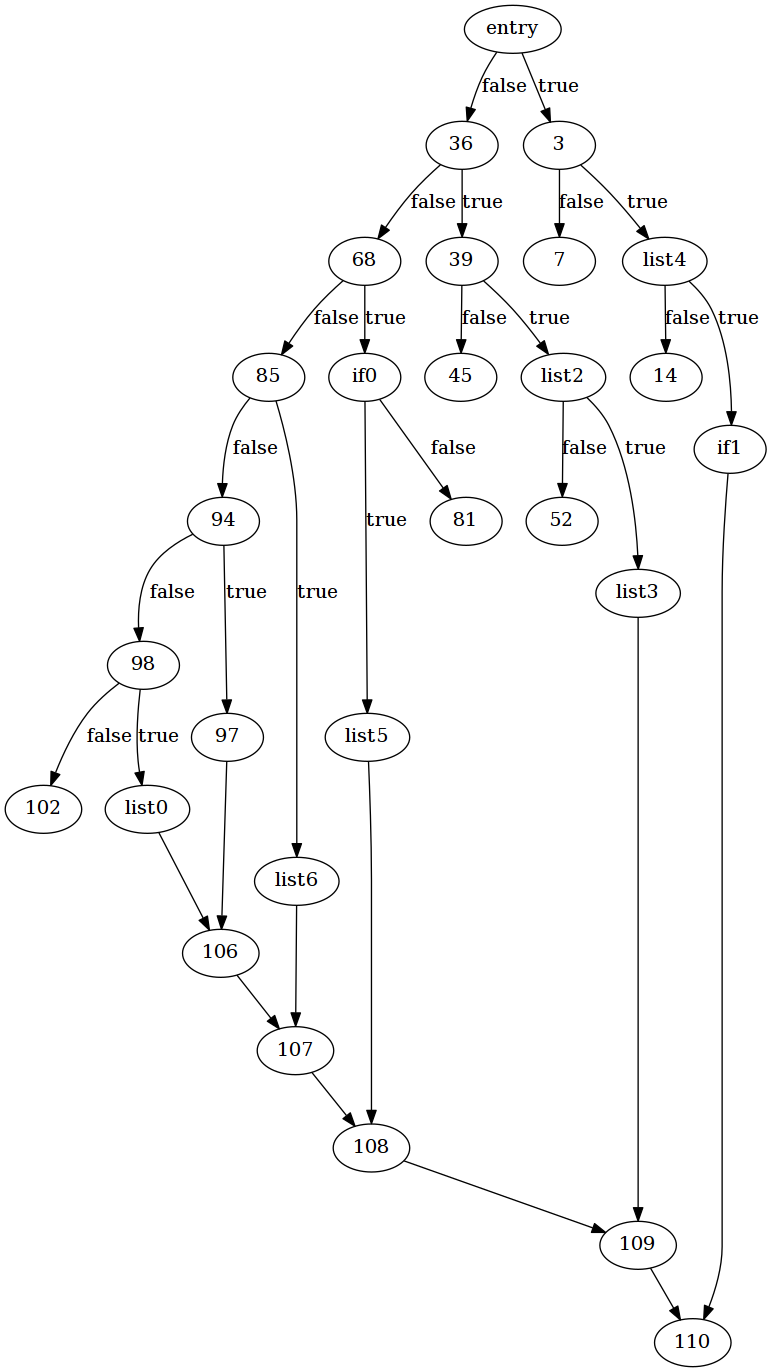
\includegraphics[width=\textwidth]{appendices/stmt_example/stmt_3.png}
	\end{subfigure}
	\caption{\textbf{Step 3}. The CFG from \textbf{step 2} (left) and a simplified CFG (right) after identifying 1-way conditionals (see figure \ref{fig:if_graph_representation}).}
	\label{fig:step_3}
\end{figure}

The fourth step further simplifies the CFG of \textbf{step 3} by recursively replacing the subgraph isomorphisms of the graph representation of 1-way conditionals with body return statements (see figure \ref{fig:if_return_graph_representation}) with single nodes, as illustrated in figure \ref{fig:step_4}.

\begin{figure}[htbp]
	\centering
	\begin{subfigure}[t]{0.45\textwidth}
		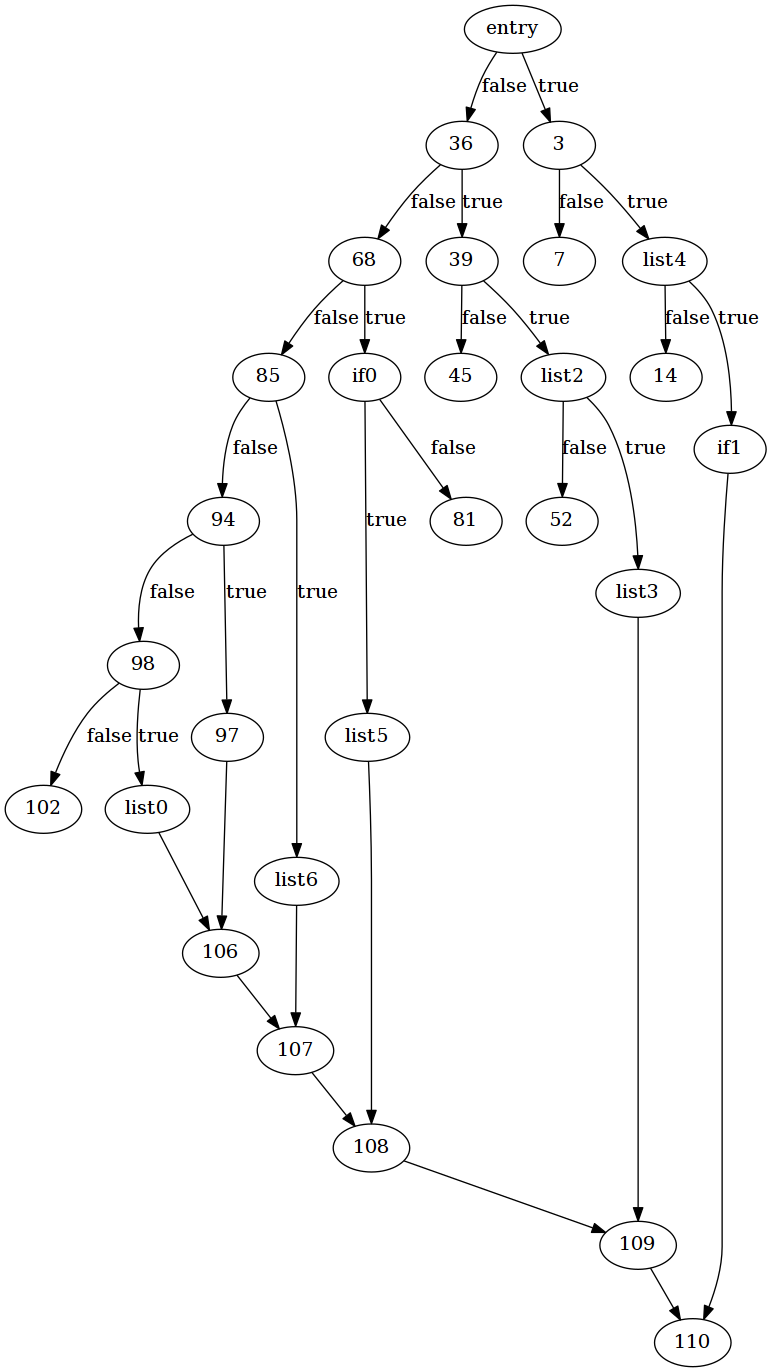
\includegraphics[width=\textwidth]{appendices/stmt_example/stmt_3.png}
	\end{subfigure}
	\qquad
	\begin{subfigure}[t]{0.45\textwidth}
		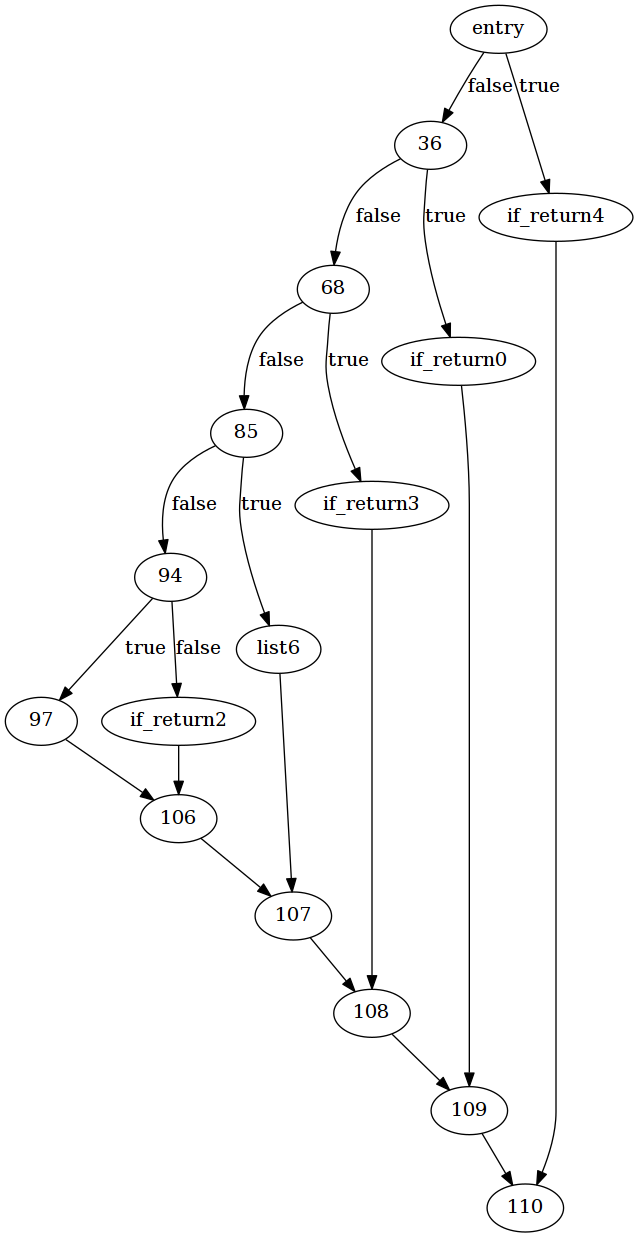
\includegraphics[width=\textwidth]{appendices/stmt_example/stmt_4.png}
	\end{subfigure}
	\caption{\textbf{Step 4}. The CFG from \textbf{step 3} (left) and a simplified CFG (right) after identifying 1-way conditionals with body return statements (see figure \ref{fig:if_return_graph_representation}).}
	\label{fig:step_4}
\end{figure}

The last step of the control flow analysis stage reduces the CFG of \textbf{step 4} into a single node by recursively replacing the subgraph isomorphisms of the graph representation of 2-way conditionals (see figure \ref{fig:if_else_graph_representation}) with single nodes, as illustrated in figure \ref{fig:step_5}.

\begin{figure}[htbp]
	\centering
	\begin{subfigure}[t]{0.45\textwidth}
		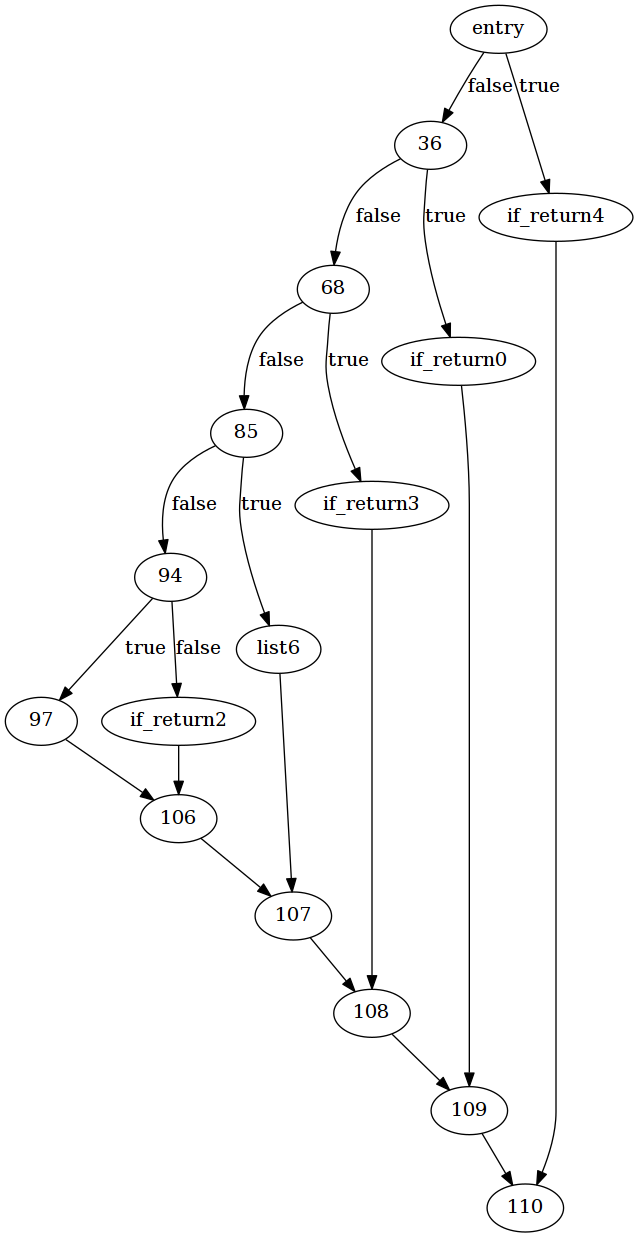
\includegraphics[width=\textwidth]{appendices/stmt_example/stmt_4.png}
	\end{subfigure}
	\qquad
	\begin{subfigure}[t]{0.45\textwidth}
		\centering
		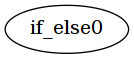
\includegraphics[width=0.3\textwidth]{appendices/stmt_example/stmt_5.png}
	\end{subfigure}
	\caption{\textbf{Step 5}. The CFG from \textbf{step 4} (left) and a simplified CFG (right) after identifying 2-way conditionals (see figure \ref{fig:if_else_graph_representation}).}
	\label{fig:step_5}
\end{figure}
